\documentclass[paper=a4, fontsize=11pt]{scrartcl} % A4 paper and 11pt font size

\newcommand{\assignment}{3}
\newcommand{\duedate}{February 15, 2023}
\usepackage[top=1in, bottom=1.5in, left=1in, right=1in]{geometry}
\usepackage{fancyhdr} % Required for custom headers
\usepackage{lastpage} % Required to determine the last page for the footer
\usepackage{extramarks} % Required for headers and footers
\usepackage[usenames,dvipsnames]{color} % Required for custom colors
\usepackage{graphicx} % Required to insert images
\usepackage{listings} % Required for insertion of code
\usepackage{courier} % Required for the courier font
\usepackage{amsmath}
\usepackage[super]{nth}
\usepackage{booktabs}
\usepackage[usenames,dvipsnames]{xcolor}
\usepackage{tcolorbox}
\usepackage{tabularx}
\usepackage{array}
\usepackage{colortbl}

%\usepackage[T1]{fontenc} % Use 8-bit encoding that has 256 glyphs
%\usepackage{fourier} % Use the Adobe Utopia font for the document - comment this line to return to the LaTeX default
\usepackage[english]{babel} % English language/hyphenation
\usepackage{amsmath,amsfonts,amsthm} % Math packages
\usepackage{graphicx}

\usepackage{hyperref}
\hypersetup{
  colorlinks   = true, %Colours links instead of ugly boxes
  urlcolor     = blue, %Colour for external hyperlinks
  linkcolor    = blue, %Colour of internal links
  citecolor   = red %Colour of citations
}

\usepackage{fancyhdr} % Custom headers and footers
\pagestyle{fancyplain} % Makes all pages in the document conform to the custom headers and footers
\fancyhead{} % No page header - if you want one, create it in the same way as the footers below
\fancyfoot[L]{} % Empty left footer
\fancyfoot[C]{} % Empty center footer
\fancyfoot[R]{\thepage} % Page numbering for right footer
\renewcommand{\headrulewidth}{0pt} % Remove header underlines
\renewcommand{\footrulewidth}{0pt} % Remove footer underlines
\setlength{\headheight}{13.6pt} % Customize the height of the header
\newcommand{\ts}{\textsuperscript}

\numberwithin{equation}{section} % Number equations within sections (i.e. 1.1, 1.2, 2.1, 2.2 instead of 1, 2, 3, 4)
\numberwithin{figure}{section} % Number figures within sections (i.e. 1.1, 1.2, 2.1, 2.2 instead of 1, 2, 3, 4)
\numberwithin{table}{section} % Number tables within sections (i.e. 1.1, 1.2, 2.1, 2.2 instead of 1, 2, 3, 4)

\setlength\parindent{0pt} % Removes all indentation from paragraphs - comment this line for an assignment with lots of text

% Default fixed font does not support bold face
\DeclareFixedFont{\ttb}{T1}{txtt}{bx}{n}{8} % for bold
\DeclareFixedFont{\ttm}{T1}{txtt}{m}{n}{8}  % for normal

%----------------------------------------------------------------------------------------
%	CODE BLOCKS
%----------------------------------------------------------------------------------------

\usepackage{adjustbox}
\usepackage{listings}
\usepackage{color}

\definecolor{dkgreen}{rgb}{0,0.6,0}
\definecolor{gray}{rgb}{0.5,0.5,0.5}
\definecolor{mauve}{rgb}{0.58,0,0.82}

\lstdefinelanguage{Dockerfile}
{
  morekeywords={FROM, RUN, CMD, LABEL, MAINTAINER, EXPOSE, ENV, ADD, COPY,
    ENTRYPOINT, VOLUME, USER, WORKDIR, ARG, ONBUILD, STOPSIGNAL, HEALTHCHECK,
    SHELL},
  morecomment=[l]{\#},
  morestring=[b]"
}

\lstset{
    columns=flexible,
    aboveskip=5mm,
    belowskip=5mm,
    keepspaces=true,
    showstringspaces=false,
    basicstyle=\ttfamily,
    commentstyle=\color{gray},
    keywordstyle=\color{purple},
    stringstyle=\color{green}
}



%----------------------------------------------------------------------------------------
%	TITLE SECTION
%----------------------------------------------------------------------------------------

\usepackage{eso-pic}
% \usepackage[demo]{graphicx}
\newcommand\AtPageUpperRight[1]{\AtPageUpperLeft{%
   \makebox[\paperwidth][r]{#1}}}

\newcommand{\horrule}[1]{\rule{\linewidth}{#1}} % Create horizontal rule command with 1 argument of height

\title{	
\normalfont \normalsize
\textsc{Northeastern University,  Khoury College of Computer Science} \\ [25pt] % Your university, school and/or department name(s)
\horrule{0.5pt} \\[0.4cm] % Thin top horizontal rule
\huge CS 6220  Data Mining \textemdash~Assignment \assignment \\ % The assignment title
\Large \textbf{Due: \duedate (100 points)} % The assignment title
\horrule{2pt} \\[0.5cm] % Thick bottom horizontal rule
}

% Original in the document
\AddToShipoutPictureBG*{%
  \AtPageUpperRight{\raisebox{-\height}{
\includegraphics[width=3cm]{images/logo}}}}

\author{
    \textbf{YOUR NAME} \\ 
    \textbf{YOUR GIT USERNAME} \\ 
    \textbf{YOUR E-MAIL}
}% INFORMATION

\date{} % Today's date or a custom date
\author{
    \textbf{YOUR NAME} \\ 
    \textbf{YOUR GIT USERNAME} \\ 
    \textbf{YOUR E-MAIL}
}% INFORMATION

\begin{document}

\maketitle % Print the title

% Convert to DOCX using https://pdf2docx.com/

{\huge \textbf{Principle Components Analysis}} \\

Italy is home to over 2000 grape varieties. Even within a single region, wines exhibit distinct attributes from different cultivators that can be measured with objective and numerical features. Notably, in the dataset we are exploring today, there are thirteen different measurements taken for different constituents found in the three types of wine. We would like to visualize how well-separated the data is for the different wineries in a 2D scatter plot.\\

We will be using the UCI Wine's dataset. Please review \verb"sklearn"'s description of \href{https://scikit-learn.org/stable/modules/generated/sklearn.datasets.load_wine.html}{wine data}, and load it in with the following code:
\begin{verbatim}
from sklearn.datasets import load_wine
wine = load_wine()
\end{verbatim} \\
\vspace{5mm}
{\Large \textbf{Question 1} [25 pts]} \\

Preprocess the the data with \textbf{z-score normalization} and scatter the data that's been projected onto the first two principle components with different colors for each target/class of wine. Include your code (linked or inline).\\

The below scatter plot is an example of displaying multiple classes with different colors on a single plot.

\begin{center}
    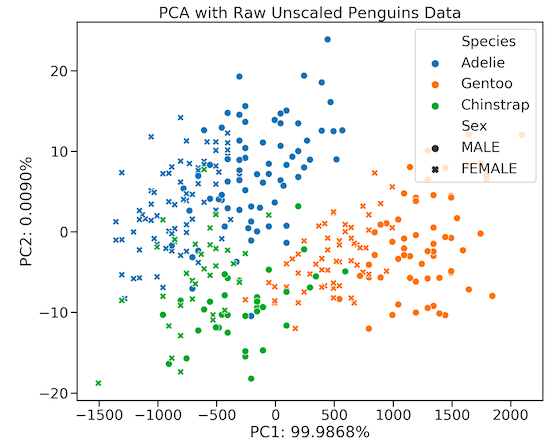
\includegraphics[width=75mm]{images/pca-example.png}
\end{center}

{\huge \textbf{Parameter Estimation}} \\

It is well-known that light bulbs commonly go out according to a Poisson distribution, and are independent regardless of whether or not they're made in the same factory. The Poisson distribution has the form: \\
\begin{equation}
p(X | \lambda) = \frac{ \exp^{-\lambda} \lambda ^{x_i}}{ x_i !} \nonumber
\end{equation} \\

An architect has outfitted a building with 32,000 of the same lightbulb. The factory has provided him with data on when $N$ of these lightbulbs have gone out over their lifetimes. They've been measured with $\mathcal{D} = \{ x_1, x_2, \cdots, x_N \}$\\
\\
{\Large \textbf{Question 2} [25 pts]} \\
\\
Derive the maximum likelihood estimate of the parameter $\lambda$ in terms of $x_i$. Please show your work. \\
\\


%%%%%%%%%%%%%%%%%%%%
{\huge \textbf{Submission Instructions}} \\
%%%%%%%%%%%%%%%%%%%%

When you have finished, follow the instructions on the \href{https://course.ccs.neu.edu/cs6220/homework-3/}{ homework main page}. Commit your code, outputs, and PDF writeup to your repository and provide the repository link to \href{https://www.gradescope.com}{Gradescope}.


\end{document}
